
\documentclass{article}

% Reduce margins to maximize image size on the page
\usepackage[margin=0.5in]{geometry}
\usepackage{graphicx}
\usepackage{subcaption}

\begin{document}
\indent Q1:\\
\\
\indent Error in Euler's method: 28.067584\\
\indent Error in Modified Euler's method: 4.768516\\
\indent Error in Improved Euler's method: 3.597160\\
\indent Error in RK4: 0.028337\\
\\
% Figure 1
\begin{figure}[htbp]
    \centering
    
\includegraphics[width=\textwidth, height=0.9\textheight, keepaspectratio]{Figure_1.png}
    %\caption{This is the caption for Figure 1.}
    \label{fig:fig1}
\end{figure}
\\
\indent Q5:\\
\\
\indent x after 50s(5000 iterations): 10.097020 (for x0=0.1, v0=1.9)\\
\indent x after 50s(5000 iterations): 54.034934 (for x0=0, v0=1.999)\\
\indent x after 50s(5000 iterations): 70.657876 (for x0=0.01, v0 =2.1)\\
\clearpage % Forces the next figure to start on a new page

% Figures 2a and 2b on the same page
\begin{figure}[htbp]
    \centering
    % Top subfigure
    \begin{subfigure}{\textwidth}
        \centering
        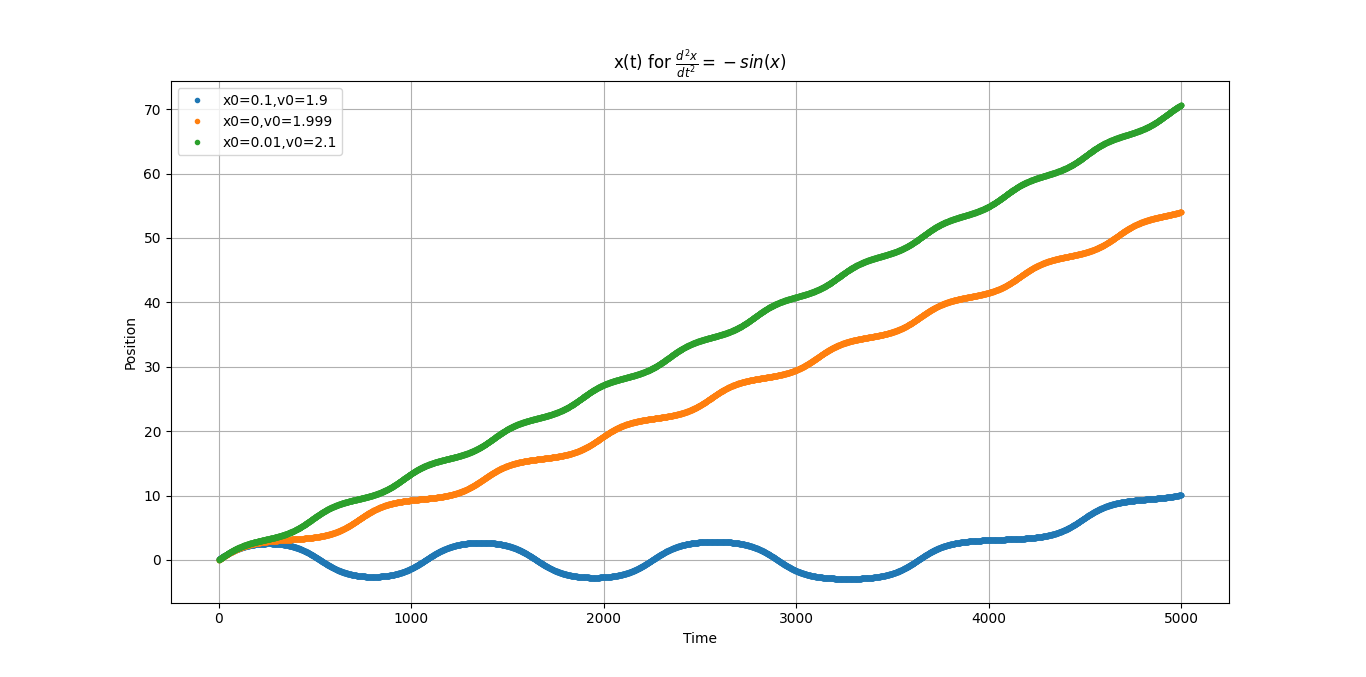
\includegraphics[width=\textwidth, height=0.45\textheight, keepaspectratio]{Figure_2a.png}
        %\caption{Caption specifically for Figure 2a.}
        \label{fig:fig2a}
    \end{subfigure}
    
    \vspace{1em} % Adds a little vertical breathing room between the images
    
    % Bottom subfigure
    \begin{subfigure}{\textwidth}
        \centering
        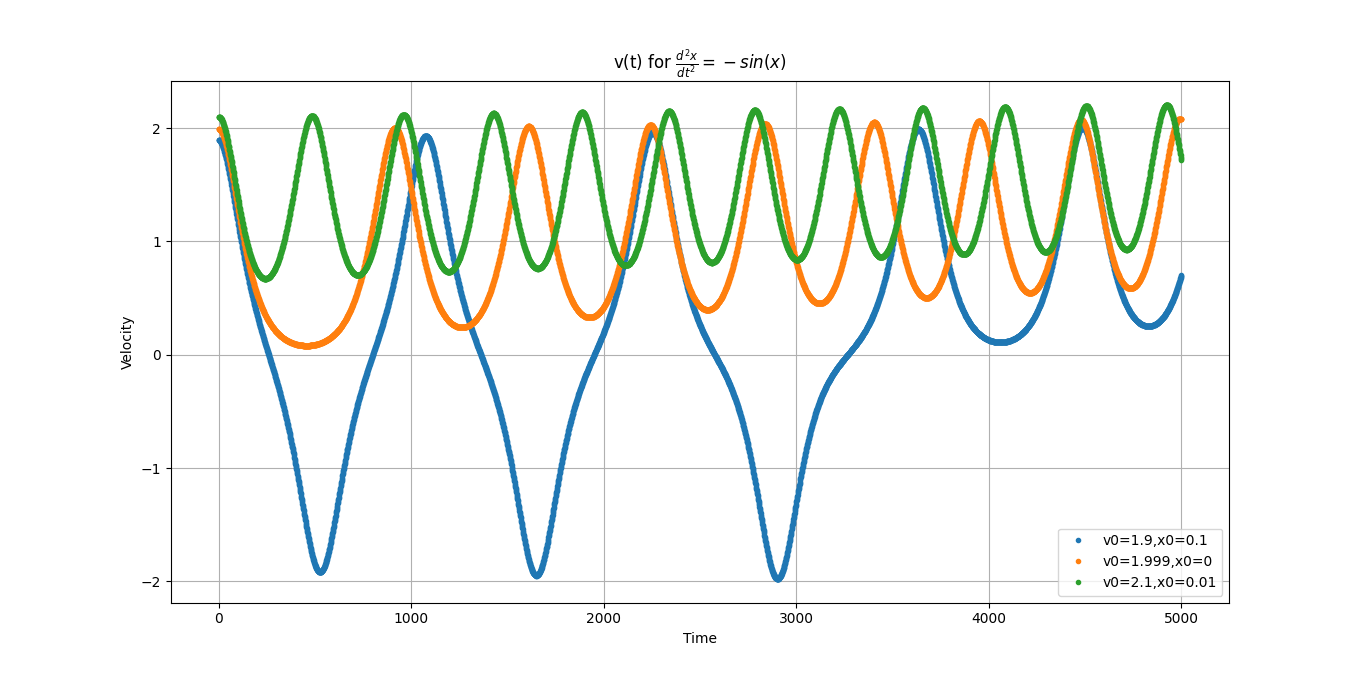
\includegraphics[width=\textwidth, height=0.45\textheight, keepaspectratio]{Figure_2b.png}
        %\caption{Caption specifically for Figure 2b.}
        \label{fig:fig2b}
    \end{subfigure}
    %\caption{Overall caption for the combined Figure 2.}
    \label{fig:fig2}
\end{figure}

\clearpage

\indent Q8:\\
\\
% Figure 3
\begin{figure}[htbp]
    \centering
    
\includegraphics[width=\textwidth, height=0.9\textheight, keepaspectratio]{Figure_3.png}
    %\caption{This is the caption for Figure 3.}
    \label{fig:fig3}
\end{figure}
\\
\indent Position of 1st particle after 2000 iterations: 0.2569\\
\indent Initial conditions: $v_{i}=0$, $y_{1} = y_{26} = 0.8$\\
\clearpage
\indent Q9:\\
\\
% Figure 4
\begin{figure}[htbp]
    \centering
    
\includegraphics[width=\textwidth, height=0.9\textheight, keepaspectratio]{Figure_4.png}
    %\caption{This is the caption for Figure 4.}
    \label{fig:fig4}
\end{figure}
\\
\indent Value of y at x=0.8: 0.233779\\
\clearpage

\indent PDE Q1:\\
\\
% Figure 5
\begin{figure}[htbp]
    \centering
    
\includegraphics[width=\textwidth, height=0.9\textheight, keepaspectratio]{Figure_5.png}
    %\caption{This is the caption for Figure 5.}
    \label{fig:fig5}
\end{figure}
\clearpage

\indent PDE Q2:\\
\\
% Figure 6
\begin{figure}[htbp]
    \centering
    
\includegraphics[width=\textwidth, height=0.9\textheight, keepaspectratio]{Figure_6.png}
    %\caption{This is the caption for Figure 6.}
    \label{fig:fig6}
\end{figure}
\clearpage

\end{document}
